\documentclass[12pt,lettersize,oneside]{article}
\usepackage[spanish]{babel}
\usepackage[utf8]{inputenc}
\usepackage{amsmath}
\usepackage{amssymb}
\usepackage{fancyhdr}
\usepackage{longtable}
\usepackage{sudoku}
\usepackage[hyphens]{url}
\usepackage{listings}
\lstset{
  language=C,
  basicstyle=\small
}
\usepackage[pdftex]{graphicx}
\usepackage{color}
\definecolor{gray75}{gray}{.75}
\lstdefinestyle{consola}
{basicstyle=\small\bf\ttfamily,
backgroundcolor=\color{gray75},
}
\lstdefinestyle{consola2}
{basicstyle=\footnotesize\bf\ttfamily,
backgroundcolor=\color{gray75},
}
\pagestyle{fancy}


\title{Grupo 3 \\Segunda versión de KECOSATS}
\author{Carlos Colmenares \and Kelwin Fernández \and Eleazar Leal}
\begin{document}
%\maketitle
\setlength{\parskip}{2.5mm}
\setlength{\itemsep}{0ex }
%\tableofcontents

\appendix
\section{Ejecución de KECOSATS}

Seguidamente daremos algunos detalles adicionales sobre la ejecución de
KECOSATS, para así ampliar la información proporcionada en le sección 5.

En la sección 5 se comentó acerca de cómo ejecutar la aplicación, repetiremos
aquí esa información, pero daremos una descripción más detallada de la entrada.


Con la distribución de KECOSATS se incluye entre otras cosas lo siguiente: \vspace{-2.5mm}
\begin{enumerate}
\item Un programa llamado {\tt sudoku} que
realiza lo siguiente:\vspace{-2.5mm}
\begin{itemize}
  \item Recibe un archivo que en cada línea tiene una instancia de Sudoku.
  \item Llama al programa KECOSATS por cada instancia.
  \item Genera automáticamente un archivo {\tt pdf} con la solución.
\end{itemize}
La idea del programa {\tt sudoku} es automatizar la prueba de los 60 casos de
uso.

\item El programa {\tt kec\_o\_sat\_s}, que en este informe hemos llamado
  simplemente KECOSATS, que resuelve instancias de SAT dadas en el
  formato DIMACS.

\item Un archivo {\tt test/sudoku.in} que tiene la lista de las 60 instancias de
  \emph{Sudoku}. La idea de incluir este archivo es suministrarlo como argumento
  al programa {\tt sudoku} para probar automáticamente los 60 casos de prueba de
  \emph{Sudoku} que contiene.
\end{enumerate}

\rule{4cm}{0.3mm}

\textbf{Paso para ejecutar la aplicación {\tt sudoku}:}
\begin{enumerate}
\item Para emplear la aplicación se debe escribir en la consola y desde el directorio
raíz, el siguiente comando tal cual

\begin{lstlisting}[style=consola]
# ./sudoku -f test/sudoku.in -o sudoku.cnf 
           -e solution.pdf -t 100
\end{lstlisting}
\end{enumerate}
donde:
\begin{itemize}
\item {\tt test/sudoku.in} Es un archivo con una lista de instancias de
  \emph{Sudoku} ---los 60 casos por ejemplo. Este archivo consiste de una serie
  de líneas de texto, cada línea representa una instancia de \emph{Sudoku} y
  tiene el formato: 
  {\tt 3 0,2,7,9,4,0,0,0,3,2,...}
  
  donde el primer número es la dimensión del \emph{Sudoku}, y le sigue una lista
  de números separados por comas, que corresponden a la asignación inicial que
  se da a las casillas de la instancia de \emph{Sudoku} a resolver. El tamaño de
  la lista de números separados por comas es el número de casillas de la
  instancia de \emph{Sudoku} que se quiere resolver.

\item {\tt sudoku.cnf} Es el archivo {\tt .cnf} que contiene la formulación
  \emph{SAT} del último caso de prueba que está contenido en {\tt
    test/sudoku.in}.
\item {\tt solution.pdf} Es el nombre del archivo {\tt .pdf} que contendrá las
  soluciones a todas las instancias codificadas en el archivo {\tt
    test/sudoku.in}.
\item{\tt 100} Es el límite de tiempo asignado a la ejecución de cada instancia
  de \emph{Sudoku}.
\end{itemize}

\rule{4cm}{0.3mm}

\textbf{Paso para ejecutar la aplicación {\tt kec\_o\_sat\_s}:}

Nota: En principio, si la idea es probar los 60 casos de prueba de \emph{Sudoku}
contenidos en {\tt test/sudoku.in}, lo ideal sería ejecutar el programa {\tt
  sudoku} tal como se indicó arriba. La ventaja es que {\tt sudoku} genera de
una vez las soluciones en {\tt pdf}.


Para emplear la aplicación, escribir en la consola el comando
\begin{enumerate}
\item \begin{lstlisting}[style=consola]
# kec_o_sat_s -f inputfilename -o outputfilename 
\end{lstlisting}
\end{enumerate}
\noindent donde:
\vspace{-2.5mm}
\begin{itemize}
\item {\tt inputfilename} es el nombre del archivo que contiene la instancia del
  problema SAT a resolver. Esta instancia debe estar en el formato DIMACS.
(Consultar http://logic.pdmi.ras.ru/~basolver/dimacs.html para información sobre
este formato.)
\item {\tt outputfilename} es el nombre del archivo que contendrá los resultados
  generados tras correr el algoritmo.
\end{itemize}


\section{Comentarios adicionales sobre el desempeño de KECOSATS}

A continuación haremos algunos comentarios complementarios acerca del desempeño
de KECOSATS con cada una de las 3 heurísticas implementadas para la selección de
la próxima variable.

 En la sección anterior que presentó la comparación de desempeño entre
  KECOSATS equipado con 3 heurísticas distintas y \emph{zChaff}, observamos
  lo siguiente:\vspace{-2.5mm}
\begin{itemize}
\item KECOSATS con la heurística \emph{greedy} se desempeñó mejor que
  \emph{zChaff} en un 46.67\% de las instancias \emph{sudoku}.
 \item Las tres heurísticas KECOSATS, \emph{BerkMin} y \emph{greedy} demoraron
   un tiempo comparable con \emph{zChaff} en casi el mismo porcentaje de veces.
\item La heurística KECOSATS es la que en un mayor porcentaje de las instancias
  está más cerca del programa que tarde menos tiempo. Esto quiere decir, que en
  las instancias en que la heurística \emph{greedy} gana en tiempo a la
  heurística KECOSATS, lo hace por una diferencia pequeña.
\item La heurística KECOSATS pudo resolver las 60 instancias de \emph{sudoku} en menos de 53 segundos. La heurística \emph{greedy}, que como hemos mencionado se desempeñó mejor en un porcentaje mayor de las instancias que la heurística KECOSATS, no pudo resolver 3 casos en menos de 70 segundos. La heurística \emph{BerkMin} por otro lado tampoco pudo resolver 1 caso en menos de 70 segundos.
\item Como la heurística KECOSATS pudo resolver todos los casos en menos de 53 segundos y en el 73\% de las instancias de \emph{Sudoku} tuvo tiempos comparables con las otras heurísticas, consideramos que es la mejor entre estas tres heurísticas.
\end{itemize}


% \begin{figure}[!ht]\caption{Número de nodos expandidos en las N-reinas, para $3 \leq
%     N \leq 13$}
% \label{NodosExpandidosReinasPeq}
% 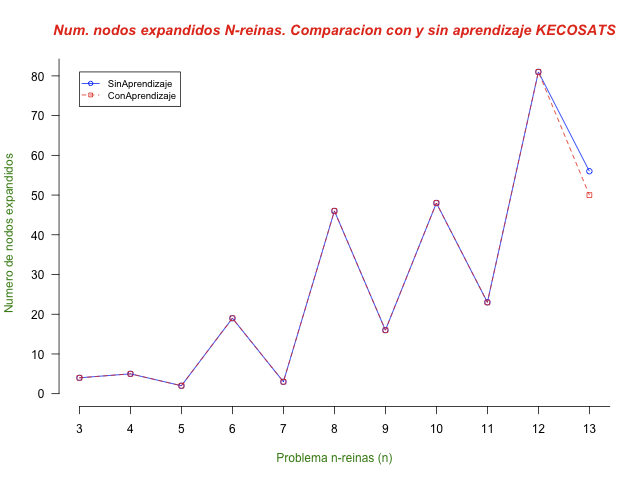
\includegraphics[scale=0.62]{figura21.png}
% \end{figure}

% \begin{figure}[!ht]\caption{Número de nodos expandidos en las N-reinas, para $14 \leq
%     N \leq 17$}
% \label{NodosExpandidosReinasPeq2}
% 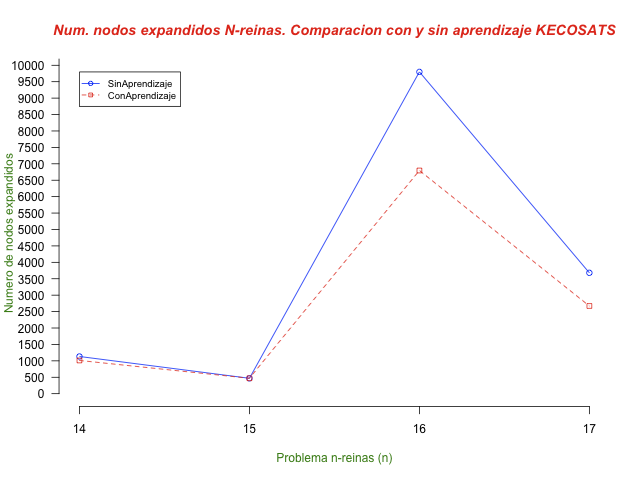
\includegraphics[scale=0.62]{figura22.png}
% \end{figure}

% \begin{figure}[!ht]\caption{Número de nodos expandidos en las N-reinas, para $18\leq
%     N \leq 29$}
% \label{NodosExpandidosReinasGrd}
% 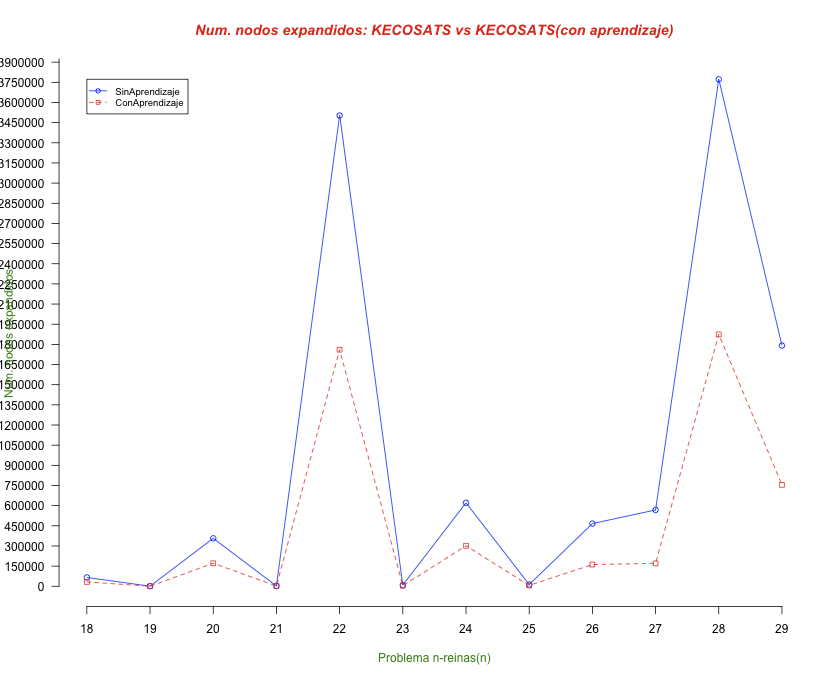
\includegraphics[scale=0.62,angle=90]{figura3.png}
% \end{figure}

\begin{center}
  \textbf{Comparación de desempeño entre las distintas heurísticas sobre la base
    del porcentaje de instancias de los 60 casos de prueba de \emph{Sudoku} en
    que determinada heurística se comportó de cierta forma. }
\end{center}
\begin{center}
\begin{tabular}{c|p{2cm}p{2cm}p{2cm}p{2.5cm}}
\hline\\\textbf{Heurística} & Mejor que \emph{zChaff} & Comparable con \emph{zChaff} & Mejor de las heurísticas & Comparable con mejor de las heurísticas \\\hline
\textbf{Greedy}     &   \textbf{46.67}\%          &  \textbf{48.33}\%   &  48.33   \%       & 71.67  \%\\
\textbf{BerkMin}    &   41.67         \% &  46.67                  \% &   28.33    \%     & 61.67 \%\\
\textbf{Kecosats}   &  40.31          \% &  46.67                  \% &    25.00
\%      & \textbf{73.33} \% \\\hline

\end{tabular}
\end{center}

Seguidamente presentamos unas tres gráficas con el objetivo de medir cuál es la cantidad de nodos que expande cada una de las heurísticas. Para ello se ejecutó KECOSATS equipado con cada una de las tres heurísticas sobre varias instancias del problema de las n-reinas (para $n=11,12,\ldots,29$) y se contó la cantidad de nodos expandidos.

Nótese que es para los casos de n-reinas grandes $n\geq 26$ que las heurísticas \emph{BerkMin} y KECOSATS empiezan a dominar a la \emph{greedy}. Este hecho se aprecia sobretodo en las instancias más difíciles de \emph{Sudoku}: a saber, la segunda y la tercera. En estas instancias de \emph{Sudoku} la diferencia de tiempo entre las heurísticas es notable, ver para ello la tabla de comparación de tiempos presentada antes.
\begin{figure}[!ht]\caption{Número de nodos expandidos en las N-reinas, para $11\leq
    N \leq 16$ por cada heurística.}
\label{NodosExpandidosReinasGrd}
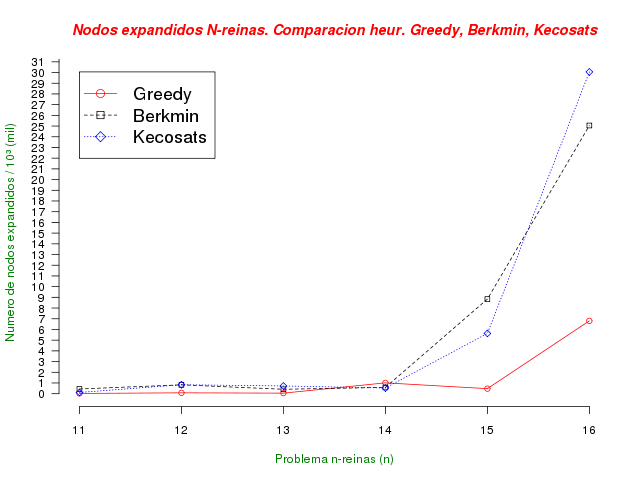
\includegraphics[scale=0.57]{reinas2Ver3.png}
\end{figure}

\begin{figure}[!ht]\caption{Número de nodos expandidos en las N-reinas, para $17\leq
    N \leq 29$. Se comparan 3 heurísticas de decisión de variable.}
\label{NodosExpandidosReinasGrd}
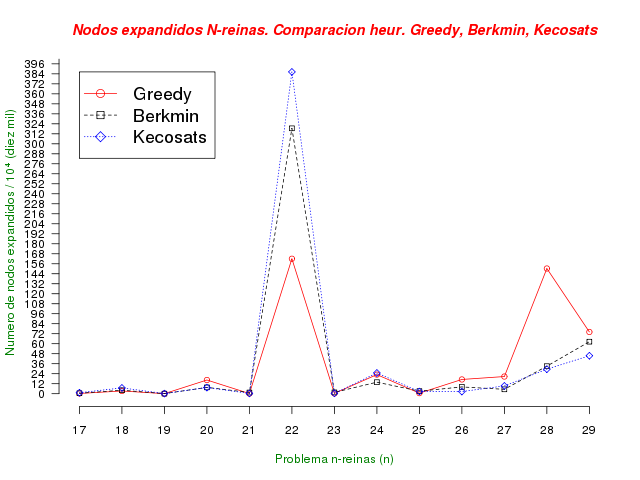
\includegraphics[scale=0.82,angle=90]{reinas3Ver3.png}
\end{figure}


\end{document}
